\documentclass{beamer}

\usepackage{amsmath}
\usepackage{amsfonts}
\usepackage{amssymb}
\usepackage{textpos}
\usepackage[orientation=portrait, size=a0,scale=1.5]{beamerposter}
\usepackage{ragged2e}
\usepackage{graphicx}

\usepackage{subfigure}


\usetheme{Berlin}
%\usecolortheme{dolphin}

\setbeamertemplate{headline}{}
\setbeamertemplate{footline}{}


\usepackage{xcolor}

% Redefine block environment background to white
\setbeamercolor{block body}{bg=white}
\setbeamercolor{block title}{bg=purple}
\setbeamercolor{title}{bg=purple}


\begin{document}
%\begin{textblock}{100}(0.1,1.6)

\title[]{\Huge Container-based high-performance computing for modeling large-scale biological neural networks  \\[-0.1 in]}
\author[]{\LARGE \textbf{Oliver James} and \textbf{Sungho Hong} \\[-0.1 in] }
\institute[]{\Large Center for Cognition and Sociality, Institute for Basic Science}
\date{}



\begin{frame}
\vspace{-0.3 in}
\maketitle

 \begin{columns}
        % First column
        \begin{column}{0.49\linewidth}
        \vspace{0 in}
            \begin{block}{\LARGE Introduction}
            \justifying
        {\large 1. Modeling large-scale, biophysically detailed neural networks increasingly relies on high-performance computing (HPC). \\[0.3 cm]

        2. However, deploying simulations of such networks across diverse HPC environments remains challenging due to software incompatibilities and complex dependencies \\[0.3 cm]

3. We address this issue using singularity containers that encapsulats the entire simulation environment, enabling neuroscientists to achieve portability and reproducibility without requiring root privileges on shared HPC systems.\\[0.3 cm]

4. We give a potential practical demonstrations using our cerebellar mossy fiber - granule cell network simulations.
               }
            \end{block}
            \vspace{0.5cm}
            \begin{block}{\LARGE Containerization for Scientific Computing}
            \centering
            \vspace{0.5cm}

\justifying
             {\large 1.  Container is a lightweight, standalone, and executable package that includes everything needed to run a piece of software  \\[0.3 cm]

              2. Run anything anywhere

               }
       \centering
               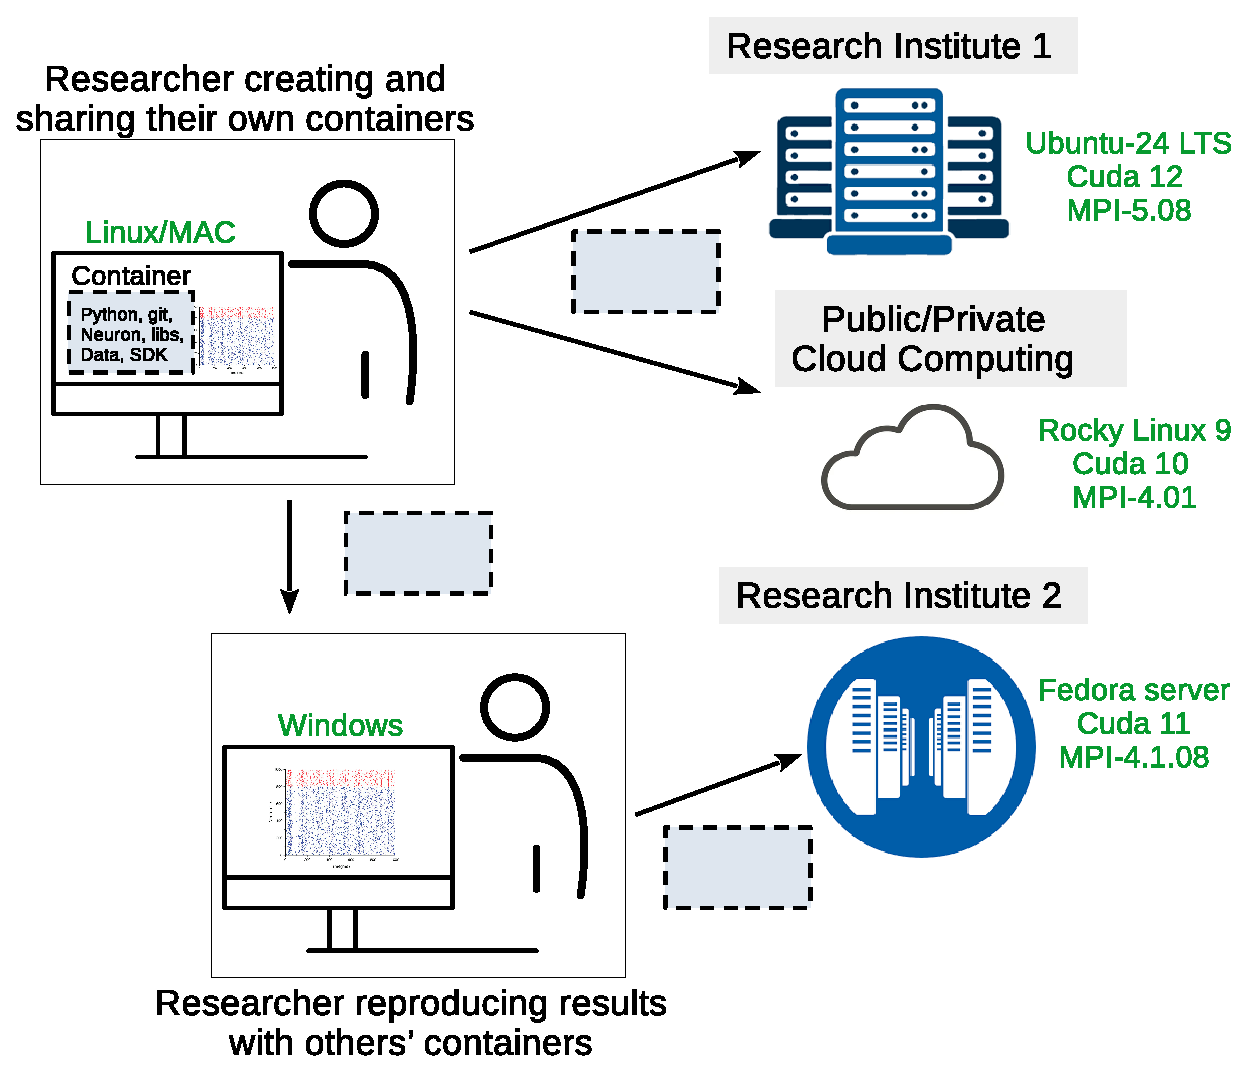
\includegraphics[scale=1.4]{output1.eps}


             %\includegraphics[scale=2.2 ]{/home/olive/Desktop/figs/tex/Paradigm_ReportOnly.eps}
            \end{block}

            \begin{block}{\LARGE Our Computational Framework}
             \vspace{2 cm}


            \centering
               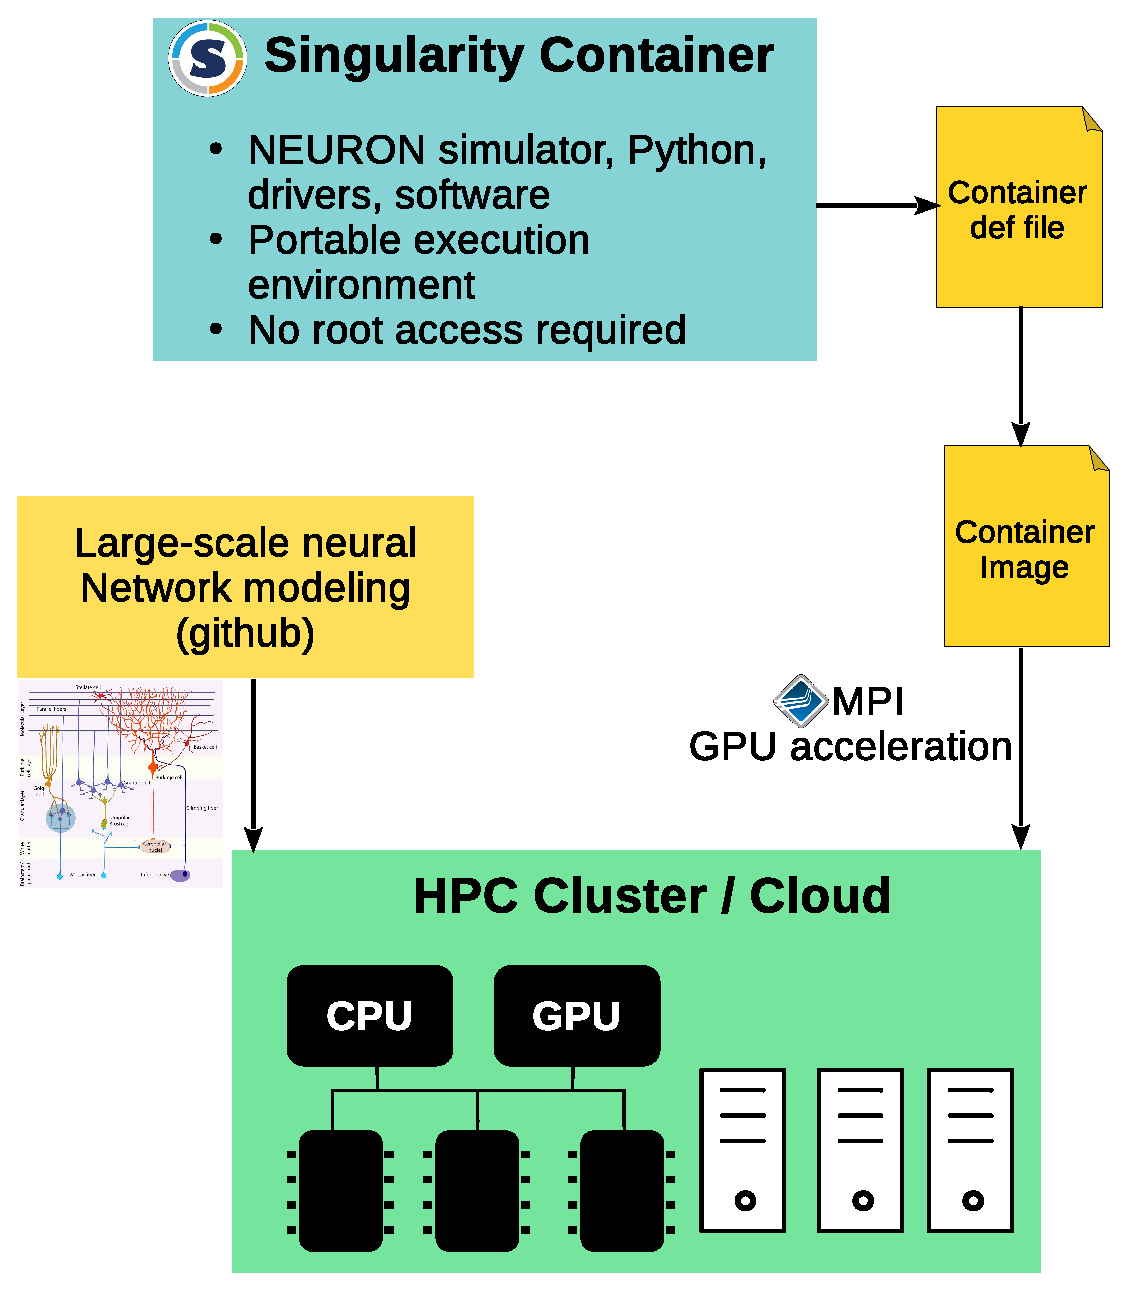
\includegraphics[scale=1.7]{output.eps}
            \end{block}



             \vspace{0.5cm}
        \end{column}

%################### Second column ####################
        \begin{column}{0.49\textwidth}
            \begin{block}{\LARGE Benchmarking Data and Network*: Cerebellar Mossy Fiber $\rightarrow$  Granule Cell}
            \centering
            \vspace{1 cm}
            \includegraphics[scale=0.45]{Cerebellum.eps}


             %\includegraphics[width=0.99\textwidth]{/home/olive/Desktop/figs/tex/PosterEEG.eps}
            \end{block}

         {\small * Nguyen, T.M., Thomas, L.A., Rhoades, J.L. et al. Structured cerebellar connectivity supports resilient pattern separation. Nature 613, 543–549 (2023)} \\[0.3 cm]

       %In visible conditions, the transition from dynamic to stable coding occurs at later time points, whereas in invisible conditions, this transition manifests earlier.



          %Visible conditions are characterized by strong dynamic neural coding, whereas invisible conditions exhibit early stable neural representations of the stimulus.




            \vspace{-0.5 cm}
            \centering
            %\includegraphics[scale=1.74,angle=-90]{/home/olive/Desktop/figs/tex/Fig2c.eps}

       \vspace{1 cm}


\begin{table}[htbp]
\centering
\caption{Network Configuration and Simulation Parameters}
\begin{tabular}{l@{\hspace{5cm}}l}
\hline
\textcolor{red}{Number of MF}         & \textcolor{red}{85600} \\
\textcolor{violet}{Number of GRC}     & \textcolor{violet}{314000} \\
Number of compartments                & 942000 \\
Number of synapses                    & 990960 \\
Simulation time                       & 2 s \\
\hline
\end{tabular}
\end{table}

 \vspace{1 cm}


            \begin{block}{\LARGE Performance Across HPC Environment}

             \vspace{0.5 cm}


\vspace{1 cm}

            \centering
            %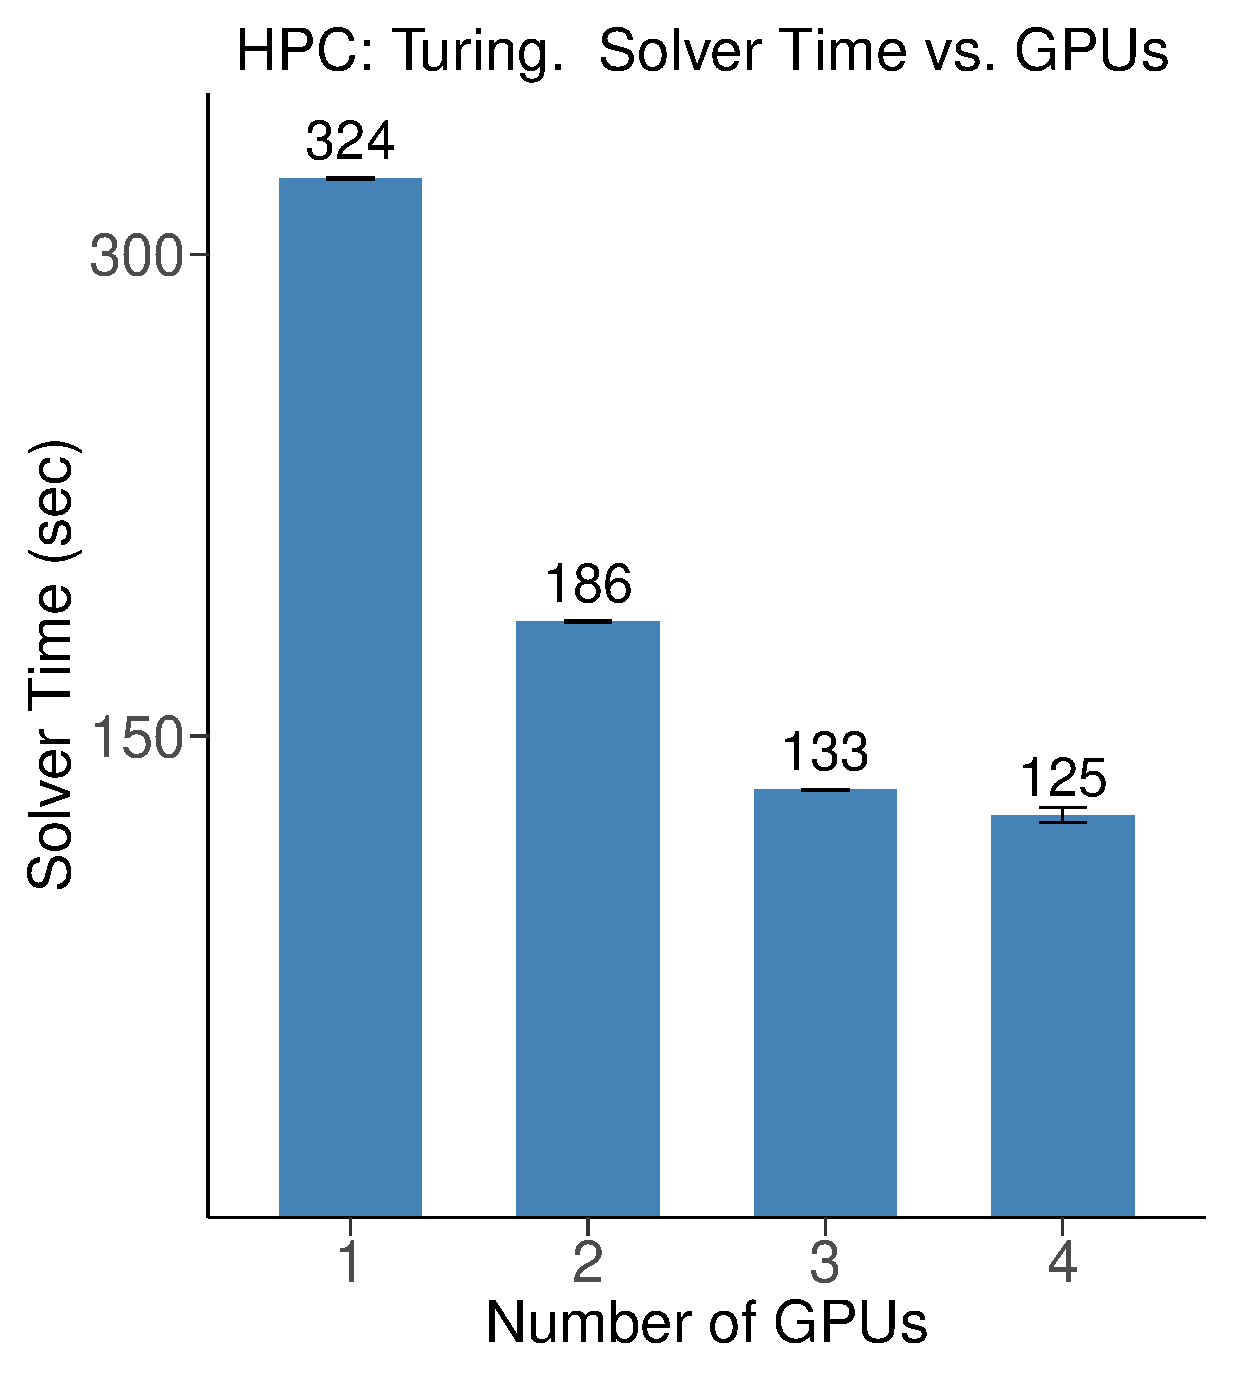
\includegraphics[width=0.45\textwidth]{Turing.eps}

            %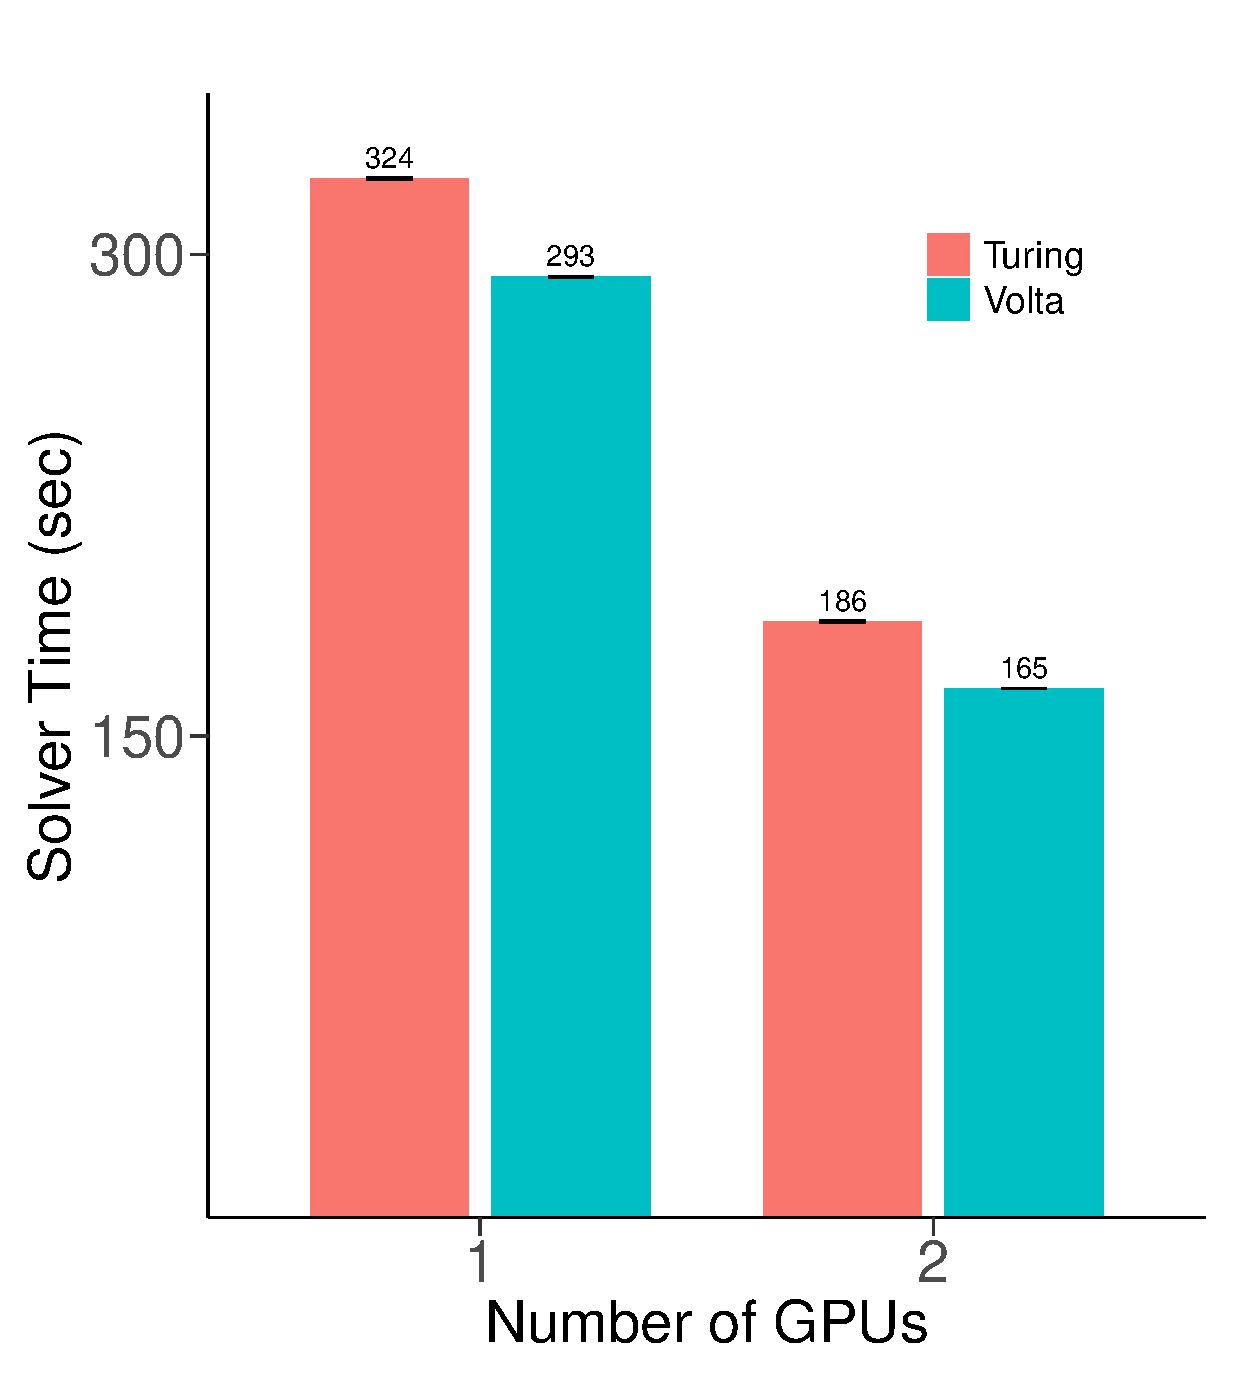
\includegraphics[width=0.45\textwidth]{HPCcompare.eps}


            \begin{figure}[htbp]
    \centering
    \begin{minipage}[b]{0.45\textwidth}
        \centering
        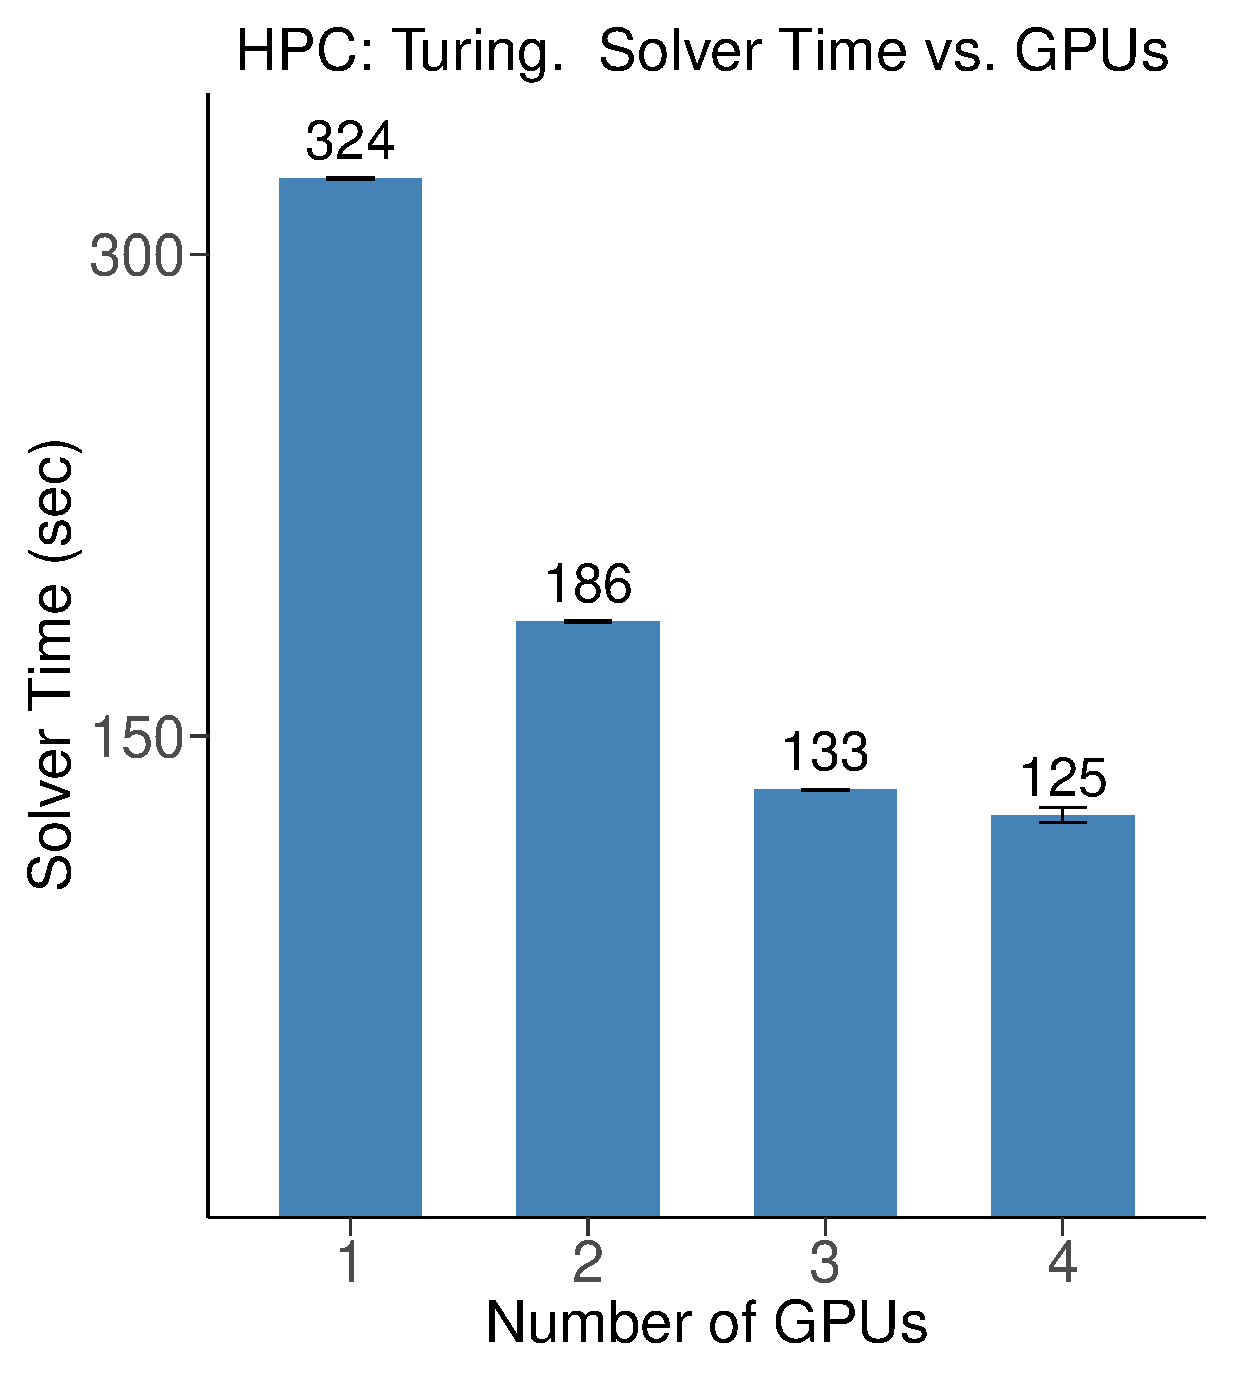
\includegraphics[width=\textwidth]{Turing.eps}
        \caption{a. Turing architecture}
        \label{fig:turing}
    \end{minipage}
    \hfill
    \begin{minipage}[b]{0.45\textwidth}
        \centering
        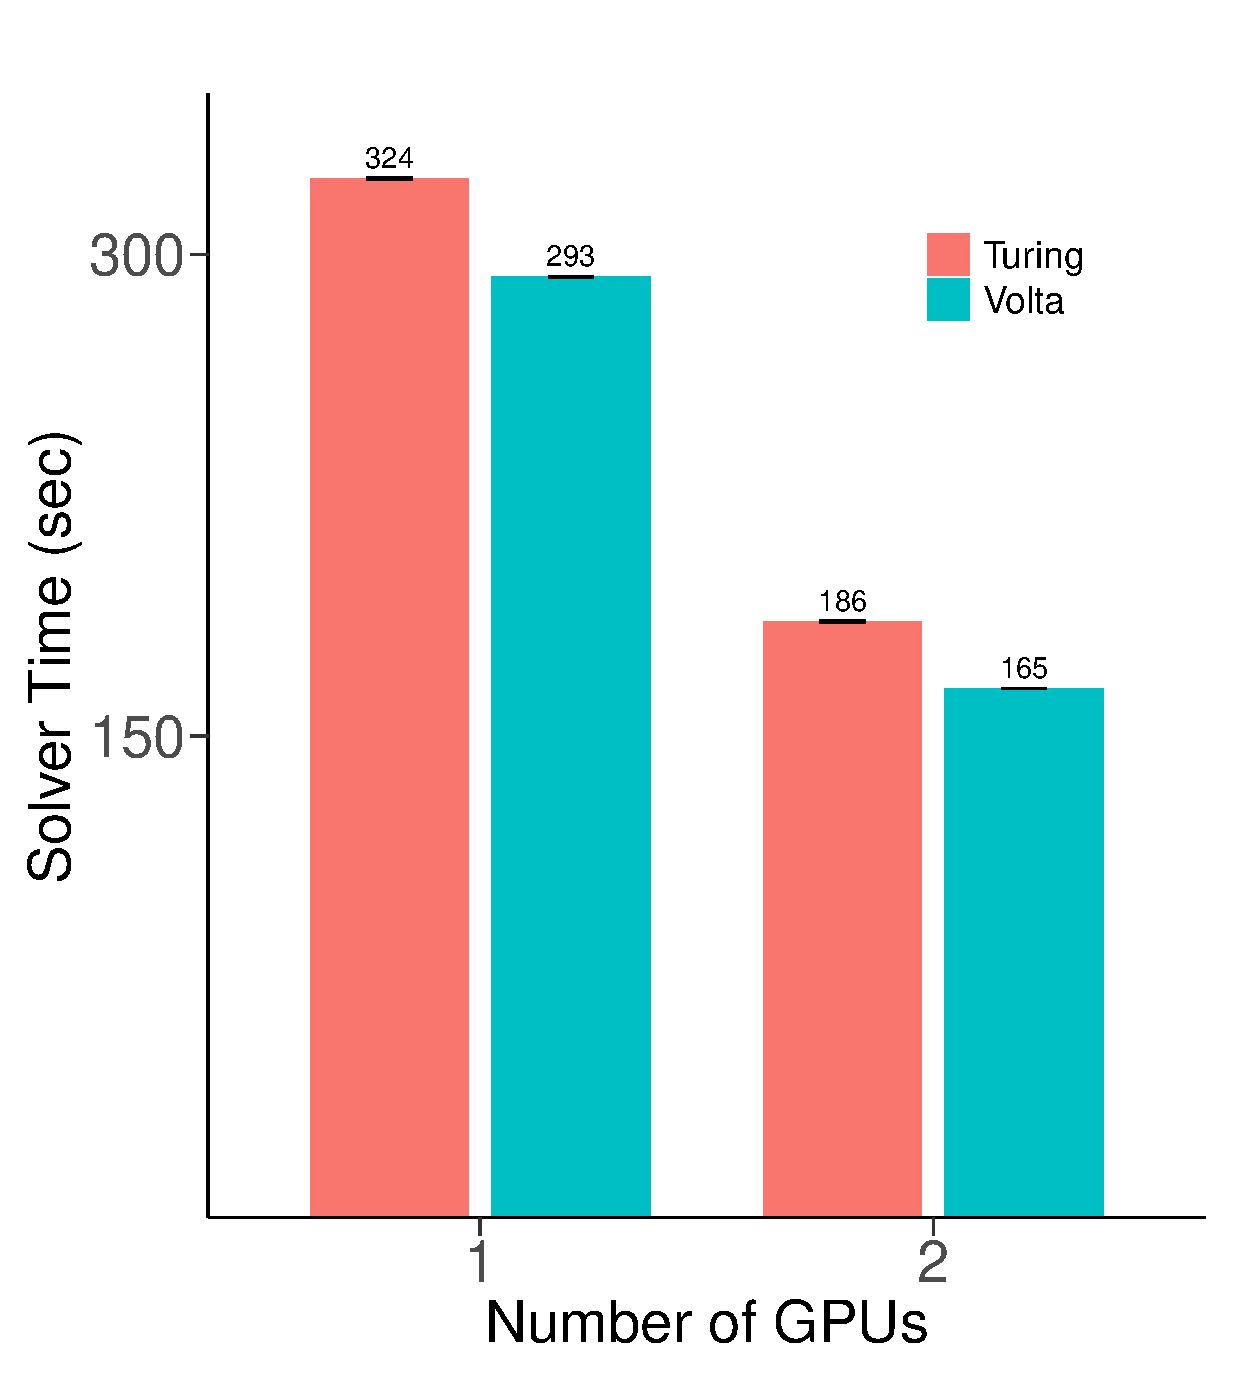
\includegraphics[width=\textwidth]{HPCcompare.eps}
        \caption{b. HPC comparison}
        \label{fig:hpccompare}
    \end{minipage}
\end{figure}


            \end{block}



             \begin{block}{\normalsize Acknowledgment}
             \justifying

This work was supported by IBS-R001-D2-2023-a00

               \end{block}

        \end{column}
    \end{columns}

\end{frame}
%\end{textblock}

\end{document}
